\documentclass[tikz, border=10pt]{standalone}
\usepackage{tikz}
\usetikzlibrary{decorations.pathmorphing, arrows.meta, shadings, calc, fadings}
\pagecolor{white}
\tikzfading[name=fade north, top color=transparent!100, bottom color=transparent!0]
\tikzset{
  atom/.style = {
    circle, shading=ball, ball color=black,
    minimum size = 32pt,
    text=white, font=\Large\bfseries\itshape,
    inner sep=0pt, outer sep=0pt
  },
  spr/.style = {
    decorate,
    decoration={coil, aspect=0.45, segment length=3.0mm, amplitude=4.5mm},
    gray!60, line width=2.0pt, line cap=round
  },
  bnd/.style  = {line width=3.5pt,  line cap=round, black!90},
  rarr/.style = {-{Stealth[length=7pt,width=5.5pt]},
                  red!90!black, line width=2.8pt},
  dbl/.style  = {{Stealth[length=7pt,width=5.5pt]}-{Stealth[length=7pt,width=5.5pt]},
                  red!90!black, line width=2.8pt}
}

\begin{document}
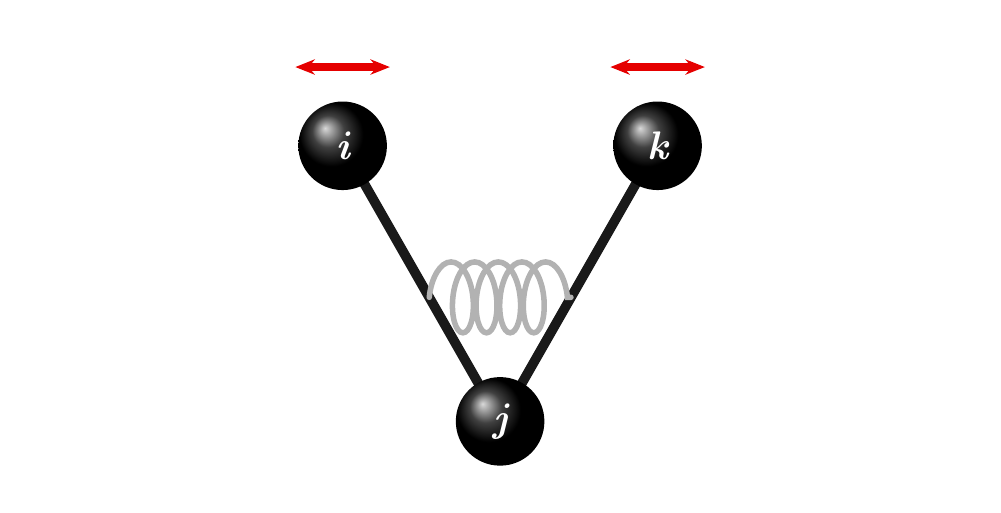
\begin{tikzpicture}
  \useasboundingbox (-6.0, -3.3) rectangle (6.0, 2.5);
  \coordinate (Pj) at ( 0.0, -2.5);
  \coordinate (Pi) at (-2.0,  1.0);
  \coordinate (Pk) at ( 2.0,  1.0);
  
  %% Bonds
  \draw[bnd] (Pi) -- (Pj);
  \draw[bnd] (Pk) -- (Pj);
  
  %% Spring between the middle of the bonds
  \coordinate (Mi) at ($(Pi)!0.55!(Pj)$);
  \coordinate (Mk) at ($(Pk)!0.55!(Pj)$);
  \draw[spr] (Mi) -- (Mk);
  
  %% Atoms
  \node[atom] (i) at (Pi) {\textit{i}};
  \node[atom] (k) at (Pk) {\textit{k}};
  \node[atom] (j) at (Pj) {\textit{j}};
  
  %% Red arrows above i and k
  \draw[dbl] (-2.6, 2.0) -- (-1.4, 2.0);
  \draw[dbl] ( 1.4, 2.0) -- ( 2.6, 2.0);
  
 
\end{tikzpicture}
\end{document}
